\section{Experiments: testing the theory}\label{sec:experiments}

Each statement of \cref{sec:theory} that a simulation can test was paired, before any comparison was computed, with a statistic, a prediction and a rule that turns the two into a verdict (\cref{app:agreement}). This section reports the comparisons that carry the argument; \cref{tab:agreement} lists all of them, and \cref{app:experiments} gives the remaining experiments.

\paragraph{Protocol.} All experiments use the model of \cref{sec:setup}. Every repeat draws a new data set from a seed derived from a hash of the scenario's parameters and the repeat index, so every number is reproducible bit for bit with the pinned library versions (\cref{app:reproducibility}). Where two arms of an experiment differ only in the learner's settings, such as the intercept, both arms use the same data sets. Standard errors are clustered by data set and error bars show two standard errors. \Cref{tab:experiments} summarises the designs.

\begin{table}[t]
\centering\small
\caption{Experiments. $K$ is the number of shadows; ``null features as shadows'' means that the strong-null columns of the data serve as the shadows, so only the false negative rate is defined.}\label{tab:experiments}
\begin{tabular}{@{}lp{0.70\textwidth}r@{}}
\toprule
 & Design & Data sets\\
\midrule
E1 & One depth-1 tree; 1 informative and 9 null features; $\nmin$ 10--1000, $p\in\{0.001, 0.01, 0.1\}$, $\delta$ 0.1--1; both intercepts; exact and \code{hist}; 100 repeats & 34{,}000\\
E2 & 300 trees; 5 relevant and 5 null features (null features as shadows, $K = 5$); $\nmin$ 10--2000, $p$ 0.001--0.2, $\delta\in\{0, 0.3, 0.5, 1\}$; both intercepts on the same data; also XGBoost 3.1 & \numEtwoFits\\
E3 & As E2, importances after $k = 1,\dots,300$ rounds & \numEthreeFits\\
E4 & 5 relevant and 5 irrelevant candidates, $K = 10$ method-built shadows, $\delta = 0.5$, $\nmin$ 10--500, $p\in\{0.01, 0.1\}$; 14 selection methods on the same data sets; 20 repeats & \numEfourFits\\
E5 & As E2 at $\delta = 0.5$ with LightGBM, random forests and scikit-learn gradient boosting & \numEfiveFits\\
E7 & E4 design, 60 Boruta rounds stored round by round & 6{,}000\\
E8 & One-shot rule with $K = 5$, 50 or 200 null features & 180\\
E9 & Eight departures from the Gaussian model (\cref{sec:robustness}) & \numEnineFits\\
E10 & Level with discrete columns: Boruta's and per-feature shadows & \numEtenFits\\
E11 & Five real tables with appended null columns (\cref{sec:realdata}) & \numEelevenFits\\
\bottomrule
\end{tabular}
\end{table}

\subsection{The first split}\label{sec:exp-first}

\paragraph{The gain is Pearson's chi-square, and the null law depends on $\nmin$ (P1--P3).} With $\lambda = 0$, exact search and the prevalence intercept, the root gain reported by XGBoost matches $X^2$ to a relative error of \numPoneErr, which is float32 precision. Under XGBoost's default regularisation, the median of a null feature's best split varies by at most \numPthreeSpread\% across $n = 10^3$ to $10^5$ at every $\nmin$ (\cref{fig:first}a), while it grows only slowly with $\nmin$. Without regularisation it grows with $n$, as remark (iii) after \cref{thm:limit} requires.

\paragraph{The limit predicts XGBoost's root decision (P4, P5).} \Cref{fig:first}b shows how often a depth-1 tree chooses the one informative feature over nine null ones, with the column order shuffled before every fit so that ties are broken at random. The curves are the limit \eqref{eq:limit}, computed by Monte Carlo without fitting anything. Over the \numPfourCells{} informative cells with the prevalence intercept and exact search, the mean absolute difference between prediction and measurement is \numPfourMAE{} and the goodness-of-fit test gives $p = \numPfourP$, so the data are consistent with the limit being exact at $\phat$ as large as 0.1 and $n$ as small as 250. Histogram search agrees as closely under assumption (H1) of \cref{cor:hist} (mean difference \numPfourMAEhist). At fixed $s$, the prevalence has no detectable effect on the root decision: a logistic regression of the per-run outcome on a spline of $\log s$ and on $\log_{10}\phat$ estimates a change of \numPfiveAME{} in the win probability per decade of $\phat$ (95\% interval \numPfiveLo{} to \numPfiveHi).

\paragraph{The intercept toll (P6).} Under the XGBoost~2.x default intercept at $\phat = 0.001$, $\nmin = 50$ and $\delta = 0.5$, exact search made no split at all in \numPsixNoSplitZeroZeroOne{} of runs; evaluating \eqref{eq:toll} on each run's own data predicts whether the first tree splits in \numPsixAgree\% of the 300 runs of this cell. \Cref{fig:toll} in \cref{app:intercept-arm} shows the toll across cells.

\begin{figure}[t]
\centering
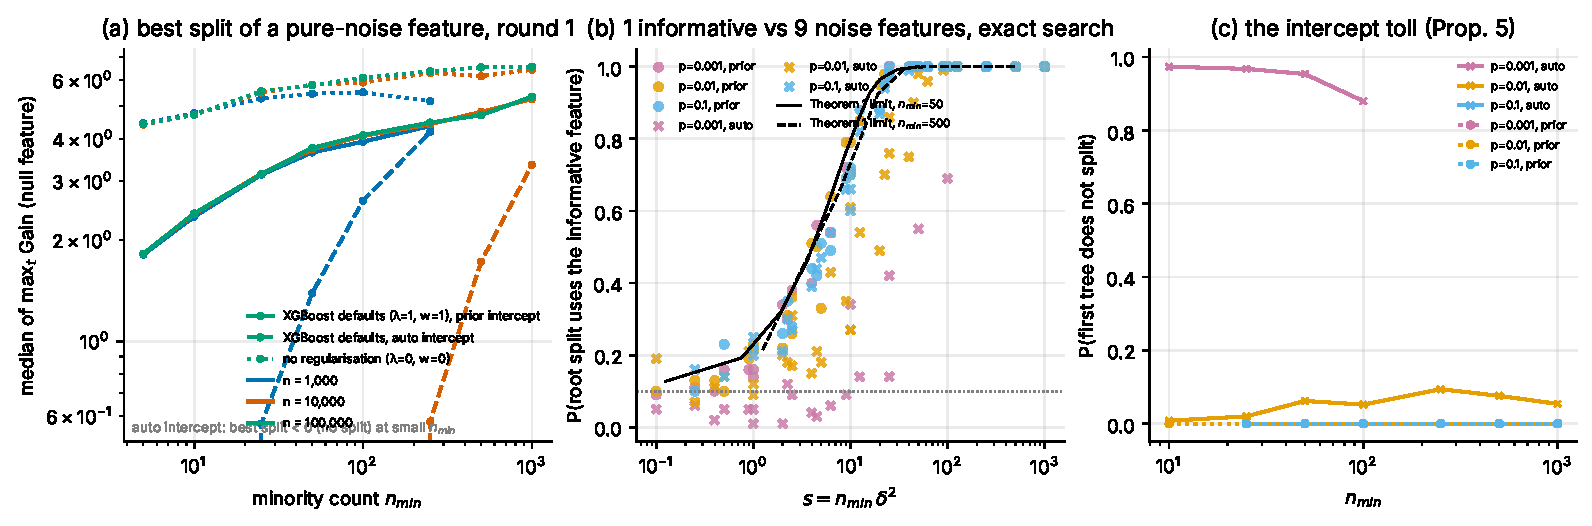
\includegraphics[width=\textwidth]{fig1_first_split}
\caption{The first split against \cref{thm:limit}. (a) Median best split of a null feature, by $n$. With XGBoost's regularisation it depends on $\nmin$ and not on $n$; without it, it grows with $n$. (b) Probability that the root uses the informative feature rather than one of nine null features (exact search, prevalence intercept), against $s = \nmin\delta^2$; error bars are two binomial standard errors. Black: the limit \eqref{eq:limit}, without fitted parameters. Dotted: chance, 1/10.}\label{fig:first}
\end{figure}

% E2, E8 and the level experiments follow once the full runs finish.
\subsection{The full ensemble}\label{sec:exp-ensemble}

\subsection{The level of the shadow rule}\label{sec:exp-level}
